% Lab 6:
% Servo Position control design project:
% Position and Rate feedbacks

\newcommand{\circscale}{0.25}

\Opensolutionfile{PosConSolutions}
% \begin{solposcon}
% \end{solposcon}

\chapter[Servo Position Control: Position \& Rate Feedbacks]{Servo Position Control Design Project:\\ Position and Rate Feedbacks} \label{ch.PosCon}

Position control systems---also known as \textit{servomechanisms} or \textit{servos}---are used extensively in industrial applications such as robot9ics and drive control.  Modern position control systems are achieved using incremental encoder sensors.  In this project you design and implement a position control system for low frequency square wave input.  By the end of the project, you should have accomplished the following objectives:
\begin{itemize}
\item
    Obtain the servo plant model.
\item
    Design a position control systems such that the output angle tracks a commanded position using position and velocity feedback.  Also, determine the feedback gains to achieve the given time-domain specifications.
\item
    Build the compensated servo plant in Simulink and simulate offline to obtain the response to a square wave input to verify the design.
\item
    Build the WinCon application, implement, and test the system on real-time hardware.
\end{itemize}

\section{Pre-Lab Assignment}

Read the following introduction and perform the calculations required to simulate the control design.  Finishing these calculations before the laboratory session is critical to finishing on time.
\par
A position control system is one that converts a position input command to a position output response.  The first step in designing any control system is to generate a mathematical model of the physical system.  In this experiment, the familiar Quanser SRV-02 plant will be our servo.  A schematic of the servomotor is shown in Figure~\ref{fig.servomotorschematic}.  Many of the pertinent characteristics of the system are quantified in Table~\ref{tab.servoparams}

\begin{figure}[bht]
\centering
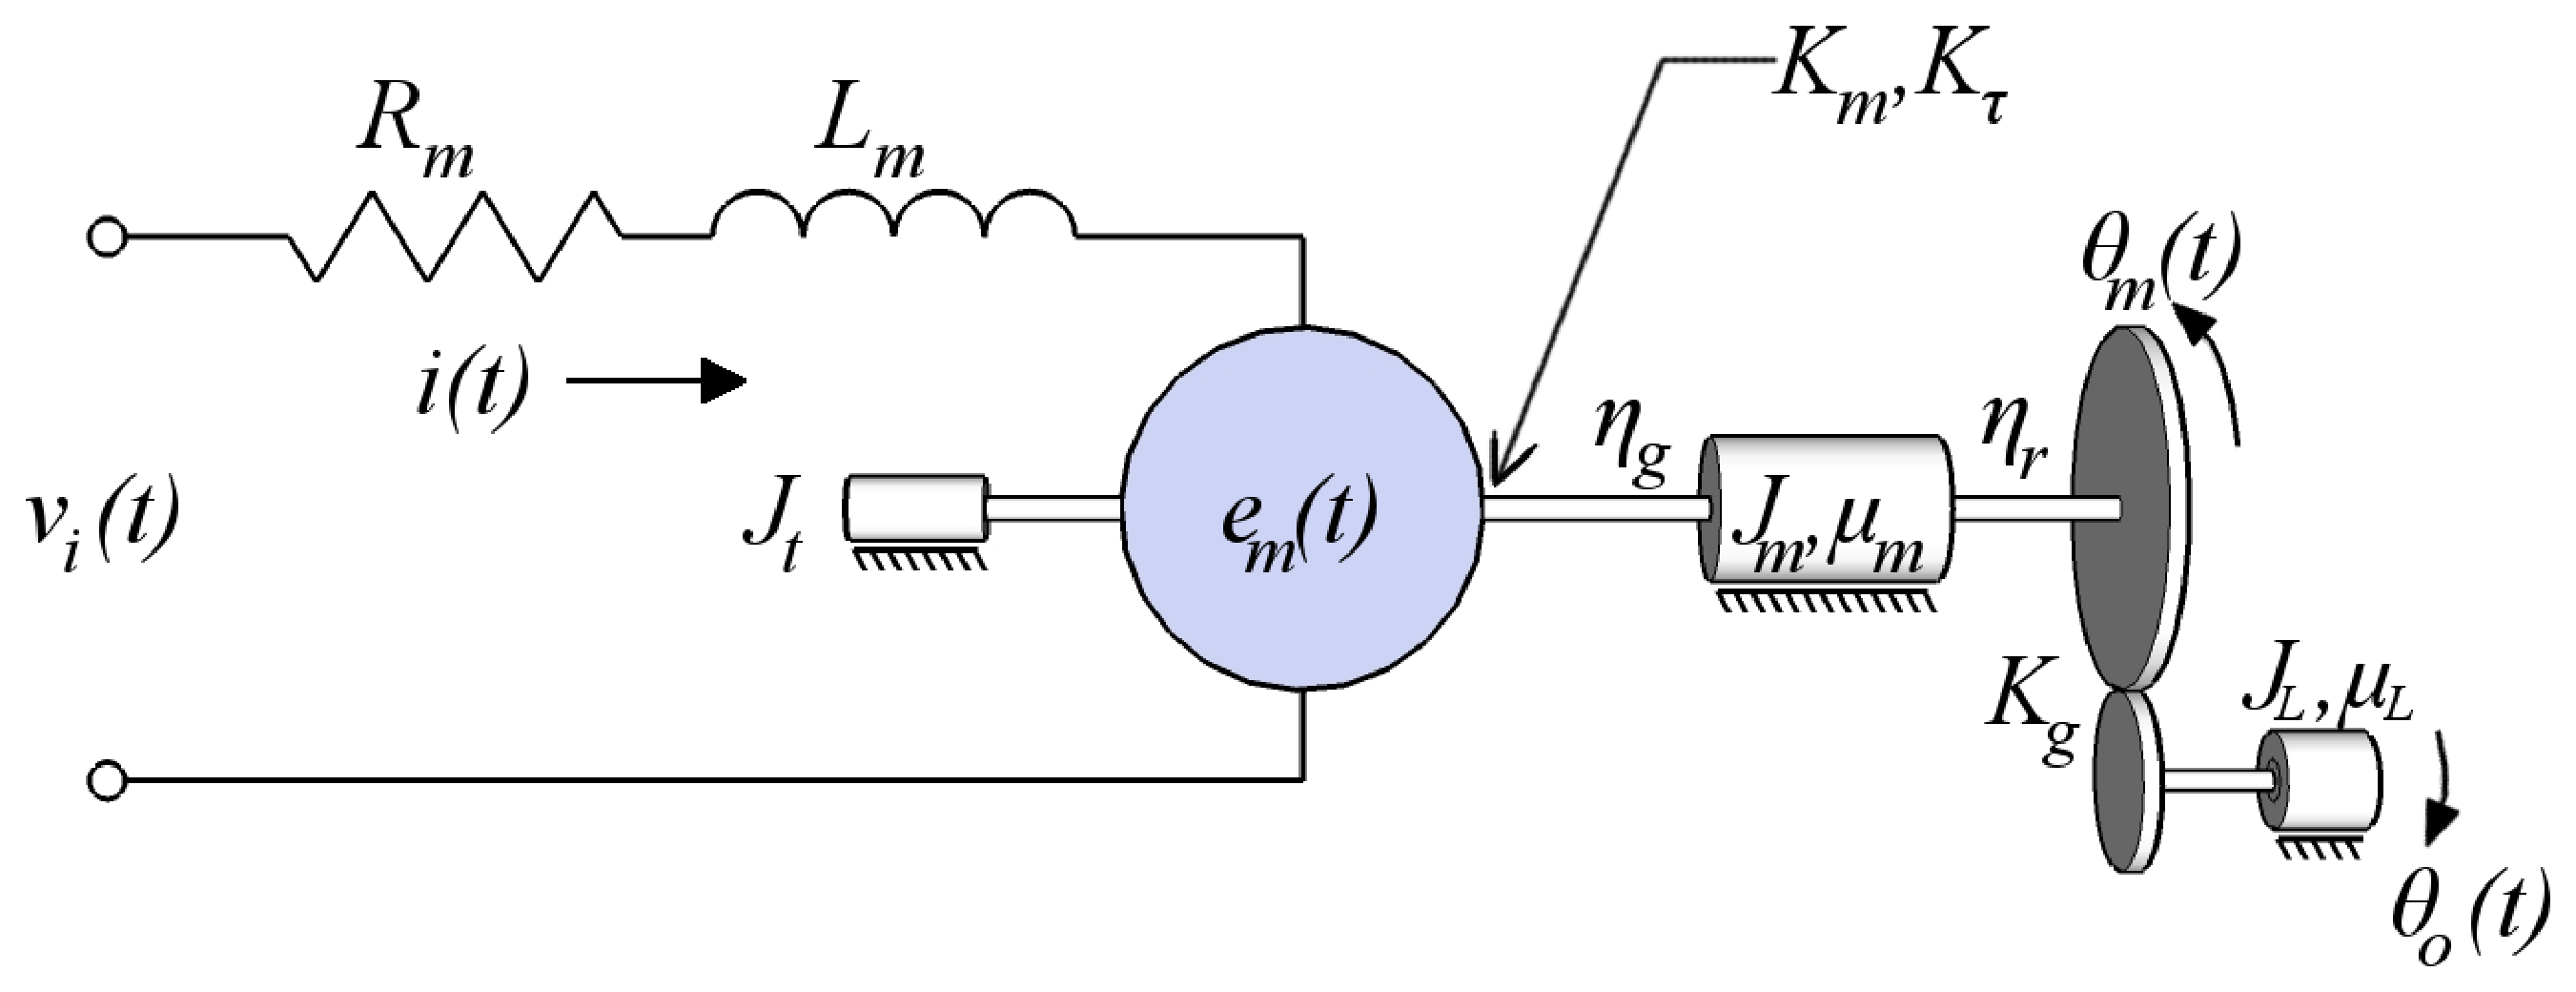
\includegraphics[scale=\circscale]{servomotor}
\caption{ \footnotesize
        Servo electromechanical schematic
        \label{fig.servomotorschematic}
        }
\end{figure}

\begin{table}[bht]
\centering \renewcommand{\arraystretch}{1.2}
\begin{tabular}{c | l | l}
    \textit{Symbol} &\multicolumn{1}{c|}{\textit{Parameter}} &
        \multicolumn{1}{c}{\textit{Value}} \\ \hline \hline
    $R_m$       &   Motor armature resistance   & $2.6\,\Omega$     \\
    $L_m$       &   Motor armature inductance   & $0.18\,$mH        \\
    $K_m$       &   Motor voltage constant      &$7.67\times10^{-3}\,$Vs/rad\\
    $K_\tau$    &   Motor torque constant       & $7.67\times10^{-3}\,$Nm/A \\
    $J_t$       &   Tachometer inertia          &
                                            $7\times10^{-8}\,\mbox{kg-m}^2$ \\
    $J_m$       &   Motor inertia       & $3.87\times10^{-7}\,\mbox{kg-m}^2$\\
    $\eta_g$    &   Gearbox efficiency          & $0.85$            \\
    $\eta_r$    &   Motor rotational efficiency & $0.87$            \\
    $K_g$       &   Transmission (gear) ratio   & $14$              \\
    $J_L$       &   Load inertia        & $1.6333\times10^{-5}\,\mbox{kg-m}^2$
\end{tabular}
\caption{\footnotesize
        Servo electric and mechanical characteristics
        \label{tab.servoparams}
        }
\end{table}
\par
Figure~\ref{fig.servomotorschematic} is a hybrid electric circuit diagram and mechanical schematic.  Looking at only the electric side, we see a fairly simply RL circuit with an input voltage $v_i(t)$ and voltage sink with emf $e_m(t)$.  In this sense, we can think of the electrical part of the servo as a subsystem (Figure~\ref{fig.servoelec}) and solve it in the frequency domain:
\begin{equation}
    I(s) = \frac{1}{R_m + L_m s} \left[V_i(s) - E_m(s)\right]
        \label{eq.servoelec}
\end{equation}
As is typical, capitalized forms of time variables represent their Laplace transforms.

\begin{figure}[bht]
\centering
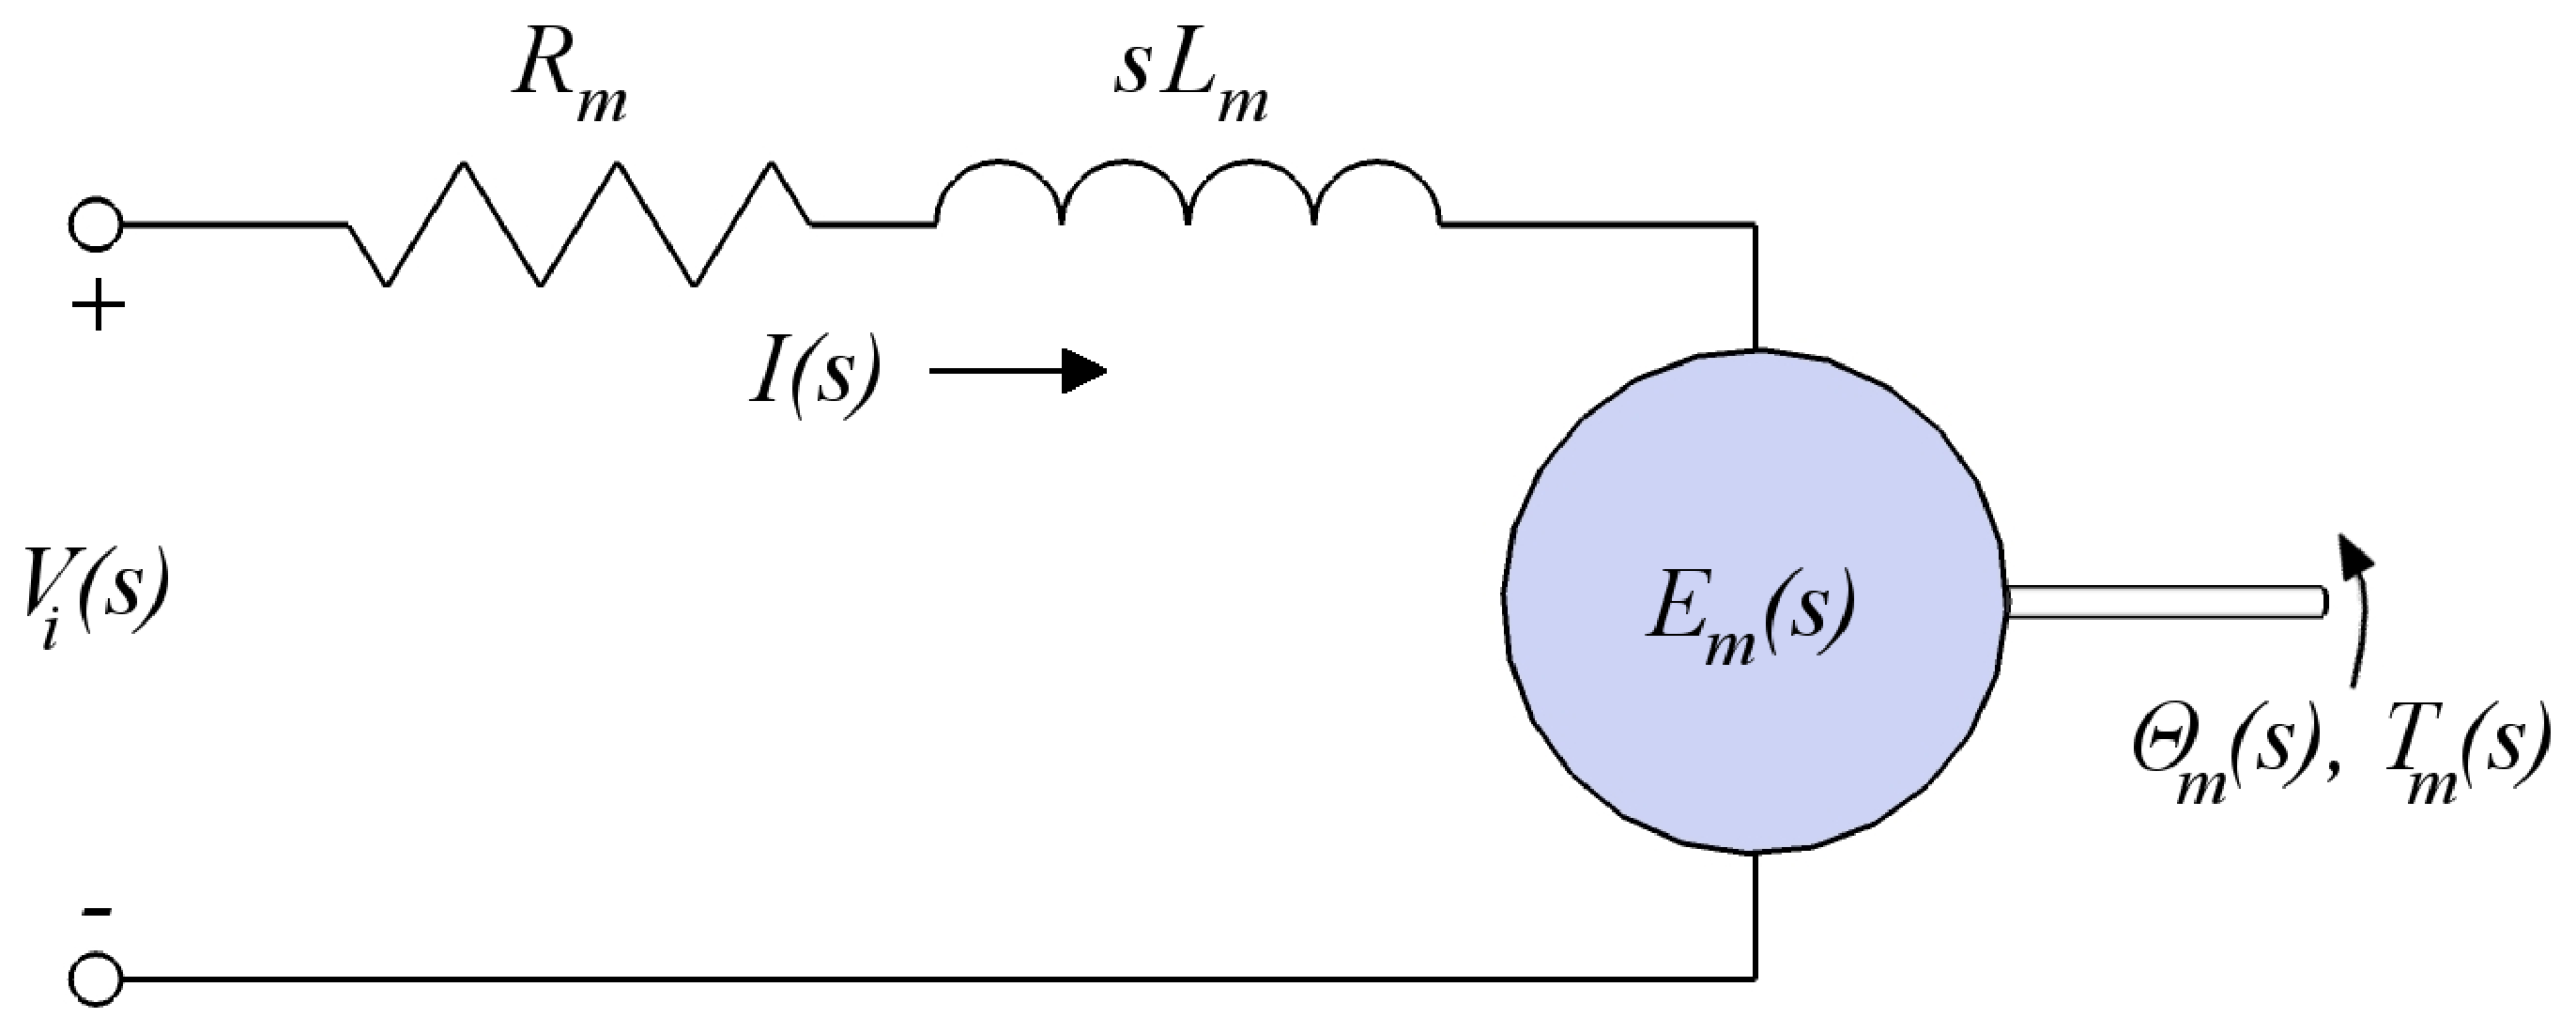
\includegraphics[scale=\circscale]{servoelec}
\caption{\footnotesize
        Servo electric circuit in the frequency domain
        \label{fig.servoelec}
        }
\end{figure}
\par
The torque produced by the motor, $\tau(t)$, is also proportional to the current, but we also must consider the losses due to gearbox inefficiency and rotational losses (like backlash).  Thus we model the motor's torque output as $\tau(t) = \eta_g \eta_r K_\tau i(t)$.  Which, in the frequency domain, is simply
\begin{equation}
    T(s) = \eta_g \eta_r K_\tau I(s)
\end{equation}
\par
The potential across the motor changes in time and is proportional to the angular velocity of the armature, $\dot{\theta}_m(t)$, and the change in the external magnetic field.  We will treat the ambient magnetic field as constant; we are left with the expression $e_m(t) = K_m \dot{\theta}_m(t)$.  Applying a Laplace transform and noting that differentiating in time is the same as multiplying by $s$ in frequency, we have:
\begin{equation}
    E_m(s) = K_m \Theta_m(s) s
\end{equation}
\par
Now that we have an expression for the output of the electric circuit in the servo---namely, the torque produced by the motor---we would like to move closer to our goal of solving for the motion of the output gear.  Again, we are looking for a closed-form expression that relates the voltage applied to the motor's circuit to the motion of the output gear (also known as the \textit{load} gear).
\par
As such, we transform the mechanical system of gears into an electric circuit analogy (see Lab~\ref{ch.ModSim} or \cite{analogs} for details on this conversion).  The analogous circuit is shown in Figure~\ref{fig.servoelecanalogy}.  For convenience, we have switched notation for the angular movement: $\dot{\theta} = \omega$ and $\mathcal{L}[\dot{\theta}] = \mathcal{L}[\omega] = \Omega(s) = s\Theta(s)$. There is a new element, however, in Fig.\ \ref{fig.servoelecanalogy}.  To represent the gear ratio between the motor and the load gears ($K_g$), we use the idea of an electrical transformer.  As an aside, the fundamental property of gears is that the ratio of parameters---including rotation speed, torque transmitted, number of teeth, and diameter---across gears is equal.  In our case, we have
\begin{equation*}
    K_g = \frac{\omega_m}{\omega_L} = \frac{T_1}{T_m} = \frac{N_L}{N_m} =
        \frac{d_L}{d_M}
\end{equation*}

\begin{figure}[bht]
\centering
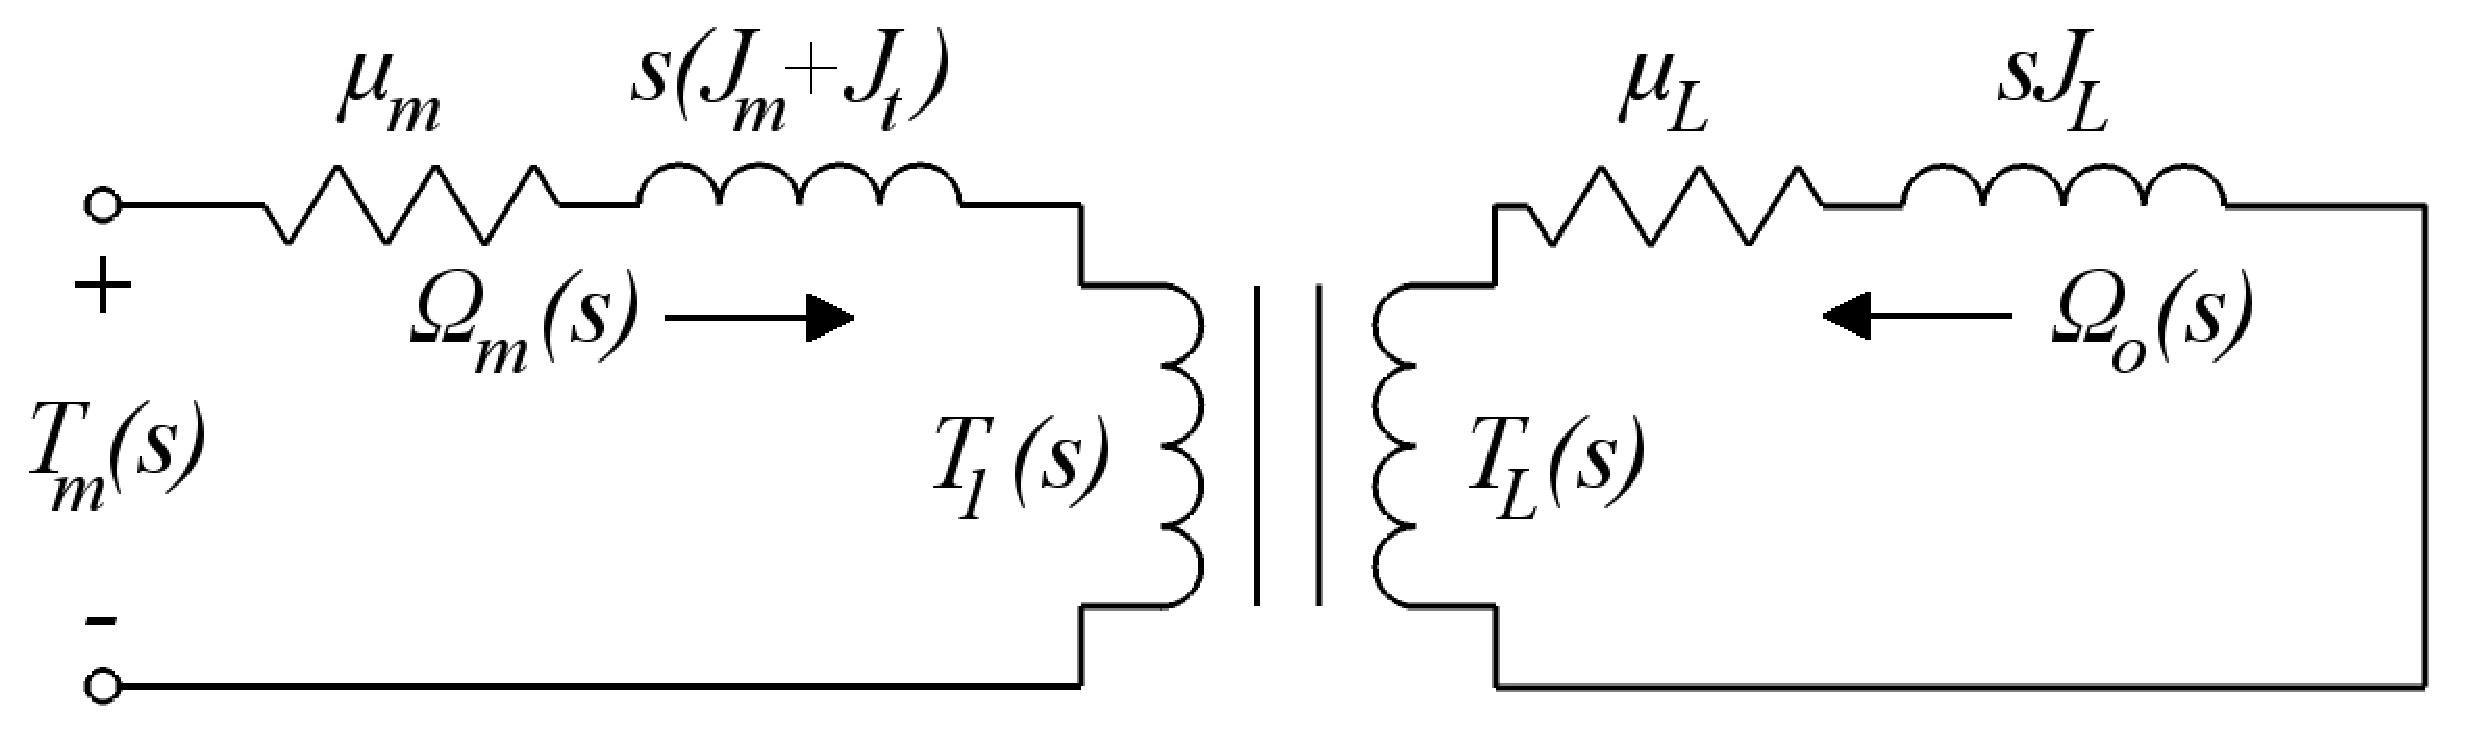
\includegraphics[scale=\circscale]{servoelecanalogy}
\caption{\footnotesize
        Electric circuit analogy for the mechanical part of the servo with quantities represented in the frequency domain.  The symbol at center is a transformer \cite{analogs}.
        \label{fig.servoelecanalogy}
        }
\end{figure}
\par
To aid in the modeling, we will now use a concept from mechanical systems to make an \textit{equivalent} system (see \cite{gears} for details).  Instead of dealing with two distinct axes of rotation (the motor shaft and the load gear shaft), we will speak instead as if all of the mechanisms were on the load shaft.  To ``move'' the motor and tachometer to the load shaft, we multiply the appropriate parameters by the square of the gear ratio and add.  Thus we get the equivalent friction and rotational inertias:
\begin{flalign*}
    \mu_{eq} &= K_g^2 \mu_m + \mu_L \approx 1\times10^{-3}\,\mbox{Nms/rad}\\
    J_{eq}   &= K_g^2(J_m + J_t) + J_L
\end{flalign*}
The equivalent system's circuit analog is shown in Figure~\ref{fig.servoelecequiv}.

\begin{figure}[bht]
\centering
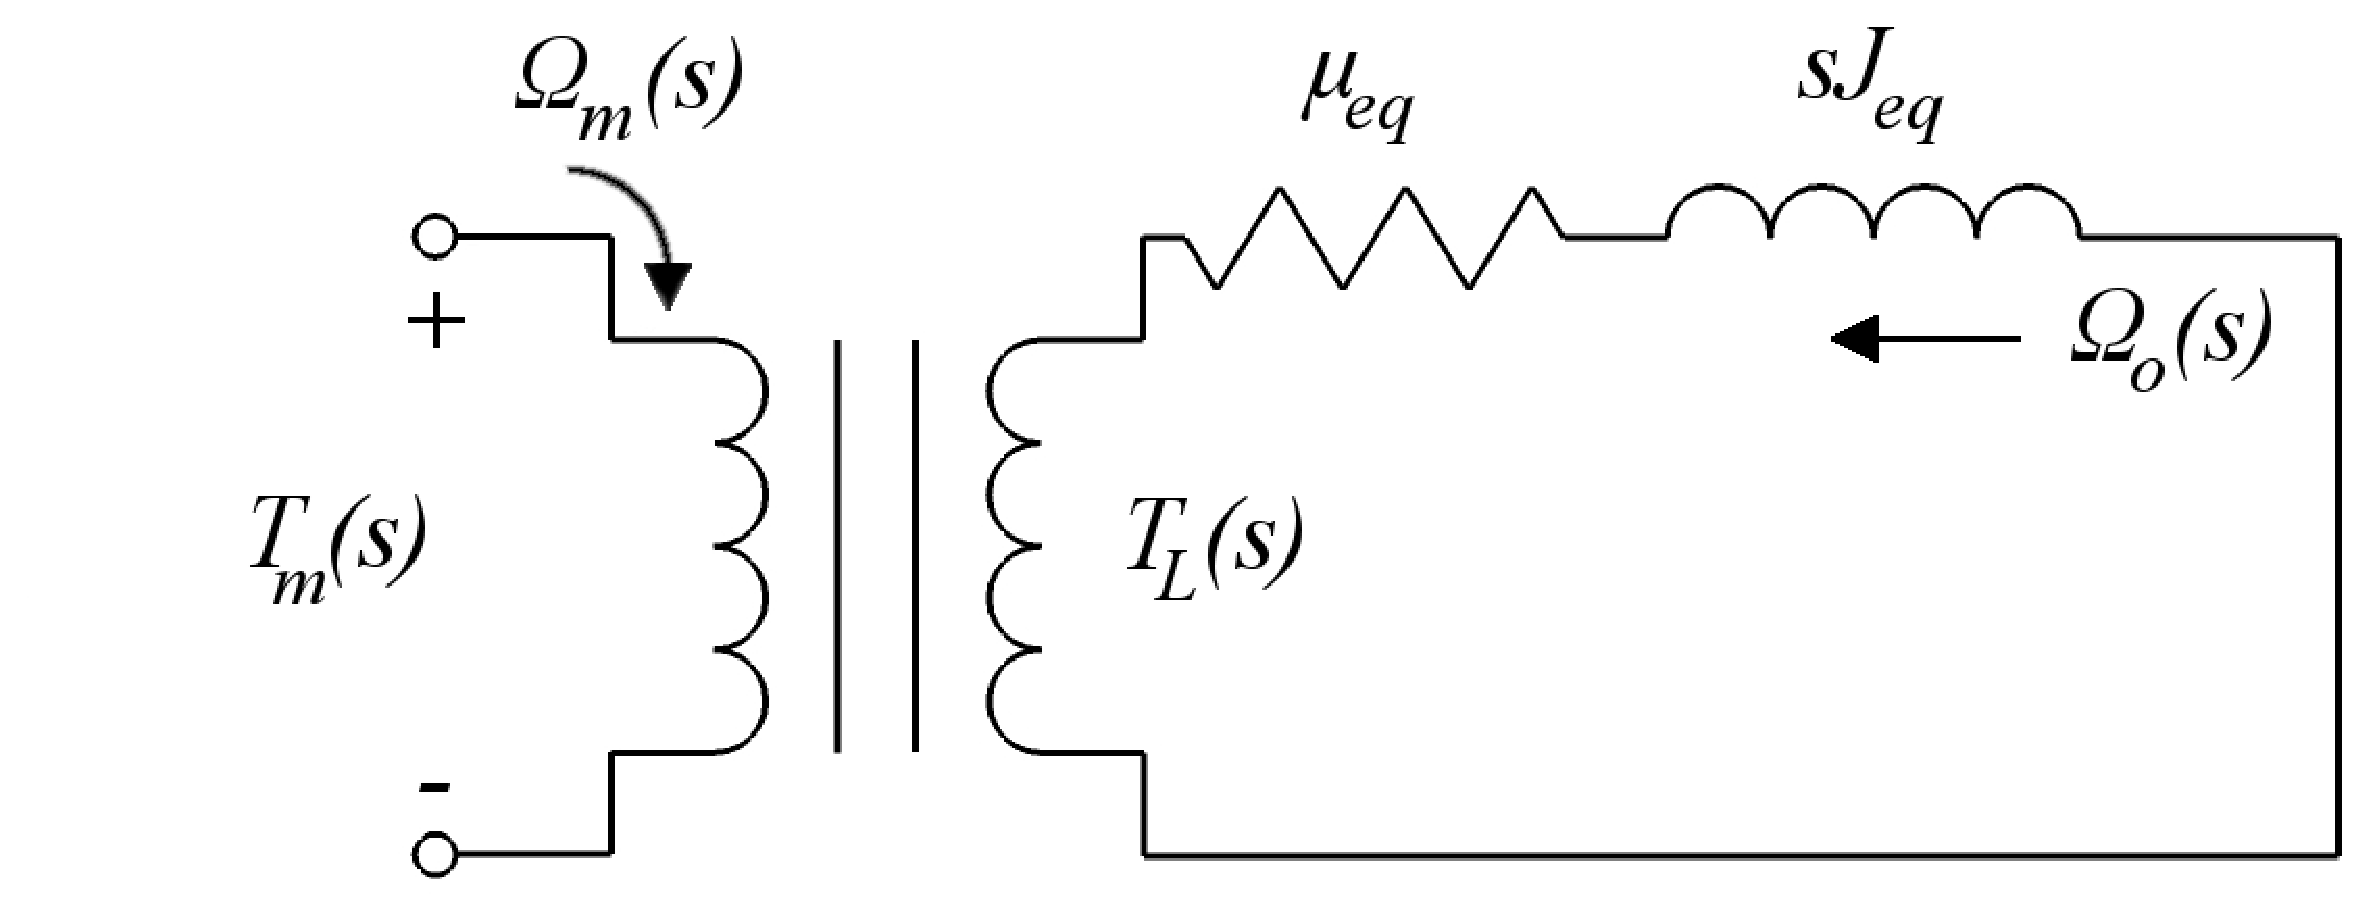
\includegraphics[scale=\circscale]{servoelecequiv}
\caption{\footnotesize
        Electric circuit analogy in the frequency domain for the equivalent mechanical system with all mechanical elements ``moved'' to the load shaft.
        \label{fig.servoelecequiv}
        }
\end{figure}
\par
From the circuit in Fig.\ \ref{fig.servoelecequiv} we have the following current relationships:
\begin{flalign}
    \Omega_o(s) & = \frac{1}{\mu_{eq} + sJ_{eq}} T_L(s) \\
    \frac{\Omega_m(s)}{\Omega_o(s)} & = K_g
        \label{eq.gearratiospeed}
\end{flalign}
\par
Using your knowledge of Laplace transforms and transfer functions, do the following:
\begin{enumerate}
\item
    Using Eqs.\ (\ref{eq.servoelec})--(\ref{eq.gearratiospeed}), draw a detailed block diagram representation for the servo system with $V_i(s)$ as input and $\Theta_o(s)$ as output.  Be sure to include all of the intermediate signals: $I(s)$, $E_m(s)$, $T_m(s)$, $T_L(s)$, and $\Omega_o(s)$.
        \begin{solposcon}
        The block diagram can be constructed by simply writing the pertinent equations one after the other and labeling the intermediate signals.  The full diagram should look something like Fig.\ \ref{fig.sol.poscon.blockdiagram}.
        \begin{figure}
        \centering
        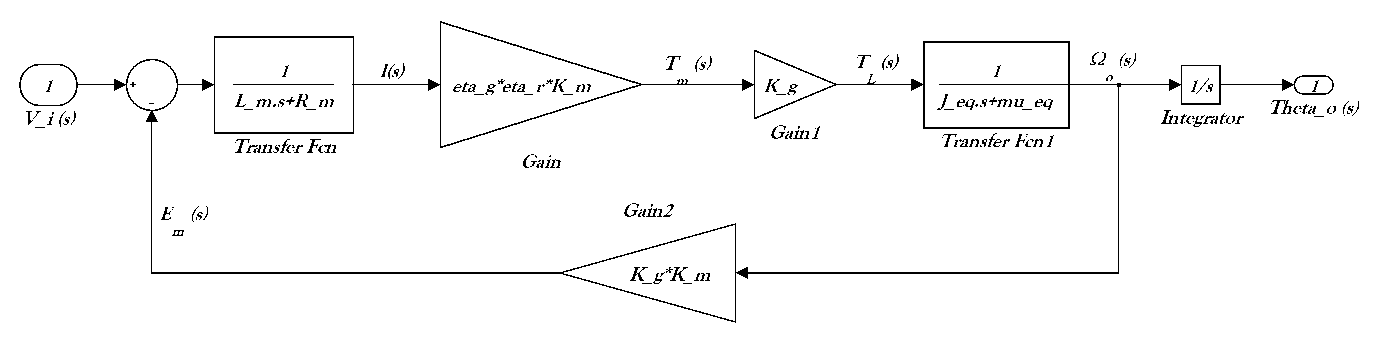
\includegraphics[angle=90, height=.95\textheight]{posconprelab1}
        \caption{\label{fig.sol.poscon.blockdiagram}}
        \end{figure}
        \end{solposcon}
\item
    We see that the motor electric time constant ($L_m/R_m$) is small compared to the mechanical time constants.  Thus, neglect the motor's electric inductance and obtain closed-loop transfer functions from $V_i(s)$ to $\Omega_o(s)$ and $\Theta_o(s)$.  You should obtain equations of the form
    \begin{flalign}
        \frac{\Omega_o(s)}{V_i(s)} &= \frac{a}{s+b} \mbox{ and } \\
        \frac{\Theta_o(s)}{V_i(s)} &= \frac{a}{s(s+b)}
    \end{flalign}
        \begin{solposcon}
        From the block diagram in question 1, it is a matter of reducing it to a single transfer function.  Use the rule that a negative feedback loop with block $G_1$ in the forward path and $G_2$ in the reverse path reduces to
        \begin{equation}
            G = \frac{G_1}{1+G_1G_2}
        \end{equation}
        After setting $L_m=0$, we have
        \begin{equation}
            TF_{V_i\to\Omega_o} =
                \frac{\frac{\eta K_m K_g}{R_m} \frac{1}{\mu_{eq} + J_{eq}s}}{ 1 + K_g K_m \frac{\eta K_m K_g}{R_m} \frac{1}{\mu_{eq} + J_{eq}s}}
        \end{equation}
        Note that $\eta := \eta_g \eta_r$.  To simplify, we multiply top and bottom of the big fraction by $\mu_{eq} + J_{eq}s$ to get
        \begin{equation}
            = \frac{
                    \frac{
                            \eta K_m K_g
                            }{
                            R_m
                            }
                    }{
                    \mu_{eq} + J_{eq}s + \frac{
                                                \eta K_m^2 K_g^2
                                                }{
                                                R_m
                                                }
                    }
        \end{equation}
        And now multiplying top and bottom by $1/J_{eq}$, we arrive at
        \begin{equation}
            = \frac{
                    \frac{
                            \eta K_m K_g
                            }{
                            R_m J_{eq}
                            }
                    }{
                    s + \frac{
                                \mu_{eq}
                                }{
                                J_{eq}
                                }
                    + \frac{
                            \eta K_m^2 K_g^2
                            }{
                            R_m J_{eq}
                            }
                    }
        \end{equation}
        Thus we have the correct form with pole-zero constants:
        \begin{subequations}
        \begin{gather}
            a = \frac{\eta K_m K_g}{R_m J_{eq}} \approx 288.3844\\
            b = \frac{\mu_{eq}}{J_{eq}} + \frac{\eta K_m^2 K_g^2}{R_m J_{eq}}
                \approx 40.4091
        \end{gather}
        \end{subequations}
        \par
        Finally, to get the TF to output position, we only need to pass the above TF through an integrator (it will have the same constants $a$ and $b$):
        \begin{equation}
            TF_{V_i\to\Theta_o} =
                \frac{a}{s(s+b)}
        \end{equation}
    \end{solposcon}
\item
    Use the Final Value Theorem to find the long-term position response to a unit step input.
        \begin{solposcon}
        The FVT looks like
        \begin{equation}
            \lim_{t\to\infty} \theta_o(t) = \lim_{s\to0}s\Theta_o(s)
        \end{equation}
        Applying this to our system, we have
        \begin{equation}
            \lim_{t\to\infty} \theta_o(t)
            =
            \lim_{s\to0} s \frac{1}{s} \frac{a}{s(s+b)} = \infty
        \end{equation}
        Some explanation:  The leading $s$ comes from the FVT itself.  The $1/s$ gives the systems response to a step input.  The rest of the expression is simply the transfer function to output position found in Question 2.
        \end{solposcon}
\item
    Now consider the servo system as a control system.  Until now, we have only had the voltage $v_i$ as the input and we simply observed its effect on the output position.  Now let us have a certain angle (position) be the input. We will obviously need some sort of conversion to turn this \textit{command} into a voltage that we can send the motor.  Call this conversion a gain and label it $K_P$.  Now the block diagram for the system looks something like Figure~\ref{fig.servoKp}.
    \begin{figure}[hbt]
    \centering
    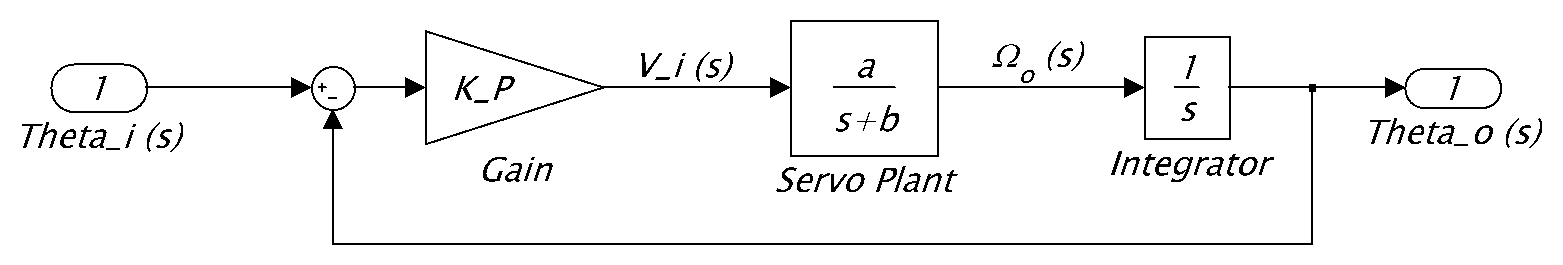
\includegraphics[width=.9\textwidth]{posconprelabKP}
    \caption{\footnotesize
            Position control block diagram with position feedback
            \label{fig.servoKp}
            }
    \end{figure}
    We call the scheme pictured in Fig.\ \ref{fig.servoKp} \textit{proportional control}.  We are able to scale the tracking error by adjusting the gain $K_P$ that gauges the voltage applied to the servo. \\
    Additionally, we can feed back the velocity signal to improve our control system's performance.  We will also run it through a gain called $K_D$.  Now the system looks like Figure~\ref{fig.servoPD}.
    \begin{figure}[bht]
    \centering
    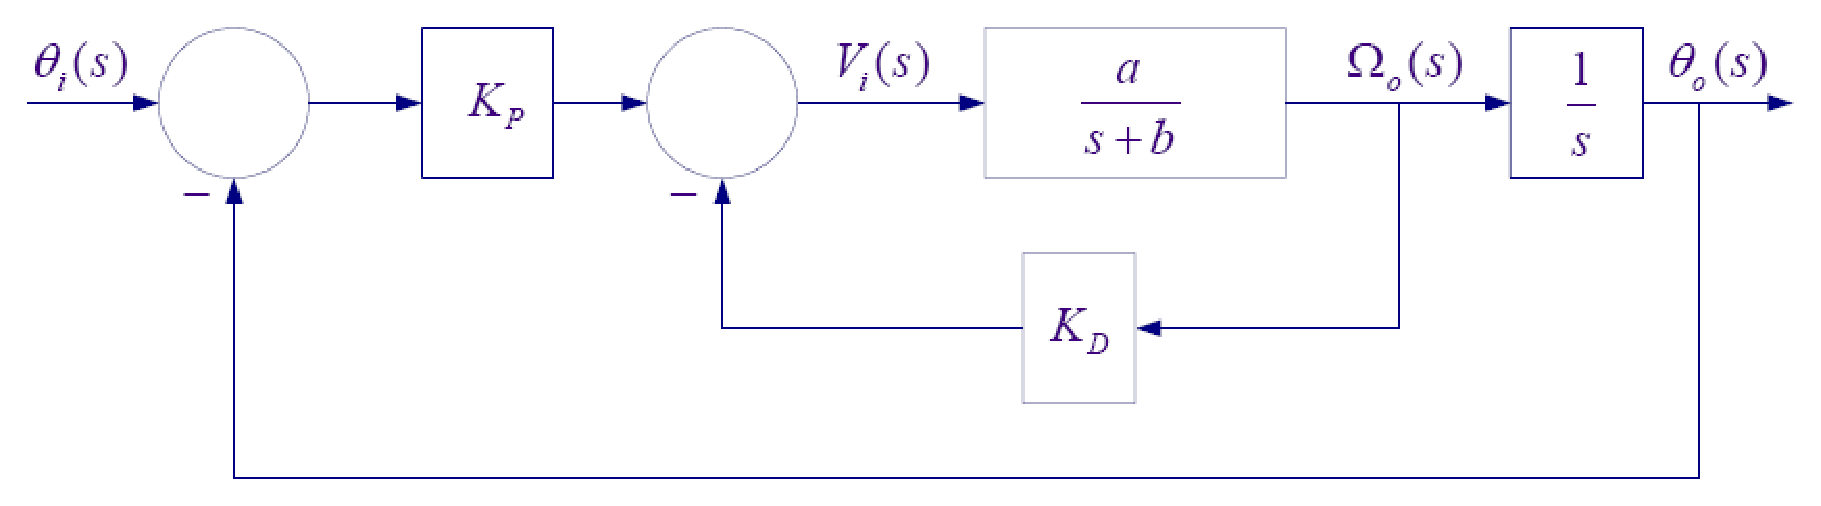
\includegraphics[width=.9\textwidth]{posconprelabPDblock}
    \caption{\footnotesize
            Position control block diagram with position and rate feedbacks (PD control).
            \label{fig.servoPD}
            }
    \end{figure}
    Find the transfer function from $\theta_i(s)$ to $\theta_o(s)$ in Figure~\ref{fig.servoPD}.
        \begin{solposcon}
        The inner feedback loop (the derivative control) in Fig.\ \ref{fig.servoPD} can be reduced to
        \begin{equation}
            G_1(s) := \frac{
                            \frac{a}{s+b}
                            }{
                            1+K_D\frac{a}{s+b}
                            }
        \end{equation}
        Then in the forward path of the remaining diagram, we have $K_P G_1(s)/s$.  The remaining diagram is a simple unity feedback system:
        \begin{equation}
            TF_{\Theta_i\to\Theta_o} :=
            \frac{K_P G_1(s)/s}{1+K_P G_1(s)/s}
                \label{eq.servoPDtf}
        \end{equation}
        Simplifying Equation~(\ref{eq.servoPDtf}) yields the classical second-order transfer function:
        \begin{equation}
            TF_{\Theta_i\to\Theta_o} =
            \frac{
                K_P a
                }{
                s^2 + s(b+K_D a) + K_P a
                }
                \label{eq.servoPD}
        \end{equation}
        \end{solposcon}
\item
    Let $\theta_i(t)$ be a square wave with amplitude 20\textdegree\ and a frequency of $1\,\mbox{Hz}$.  Determine the values for the gains $K_P$ and $K_D$ in Fig.\ \ref{fig.servoPD} such that the following time-domain specifications are met:
    \begin{itemize}
    \item A damping ratio, $\zeta = 0.707$
    \item A peak time of $t_p = 0.05\,\mbox{seconds}$.
    \end{itemize}
    For your reference, the peak time of a second-order system is given by
    \begin{equation}
        t_p = \frac{\pi}{\omega_n \sqrt{1-\zeta^2}}
    \end{equation}
    and the theoretical peak value of the response to a step input is
    \begin{equation}
        M_p = \left(1 + e^{\frac{
                                -\zeta \pi
                                }{
                                \sqrt{1-\zeta^2}
                                }
                                }
                \right) \max \theta_i
    \end{equation}
    Note that the servo's PD transfer function has the same form as the standard second-order transfer function:
    \begin{equation}
        \frac{\Theta_o(s)}{\Theta_i(s)}
        =
        \frac{
                K\omega_n^2
                }{
                s^2 + 2\zeta\omega_n s + K\omega_n^2
                }
            \label{eq.secondordertf}
    \end{equation}
        \begin{solposcon}
        Comparing Eqs.\ (\ref{eq.secondordertf}) and (\ref{eq.servoPD}), we can conclude the following basic parameters:
        \begin{subequations}
        \begin{flalign}
        K &= 1 \\
        \omega_n &= \sqrt{K_P a} \\
        \zeta &= \frac{b+K_D a}{2\sqrt{K_P a}} \label{eq.servoDR}
        \end{flalign}
        \end{subequations}
        We then translate the formula given for peak time into one with our parameters:
        \begin{equation}
        t_p =  \frac{\pi}{\omega_n \sqrt{1-\zeta^2}}
        = \frac{
                \pi
                }{
                \sqrt{K_P a}\sqrt{1-\frac{
                                        (b+K_D a)^2
                                        }{
                                        4K_P a
                                        }
                                        }
                }
            \label{eq.servoPT}
        \end{equation}
        Now we have a system of equations with two unknowns ($K_P$, and $K_D$) and two equations (\ref{eq.servoDR} and \ref{eq.servoPT}).  You can solve these using your favorite method.  One way would be to rearrange Eq.\ \ref{eq.servoDR} for $K_D$ and then substitute into Eq.\ \ref{eq.servoPT} to solve for $K_P$ first.  Using $K_P$, you can then go back and find $K_D$.
        \par
        These parameters turn out to be:
        \begin{flalign*}
            K_P &\approx 27.3708 \\
            K_D &\approx 0.2955
        \end{flalign*}
        \end{solposcon}
\item
    Create a Simulink model of the PD control system we have just derived.  Use the values for $a$, $b$, $K_P$, and $K_D$ from above.  The Simulink model should look similar to Figure~\ref{fig.servoPDmodel}.  Change the simulation parameters to a``Fixed-step'' of 0.001 and ``ode4 (Runge-Kutta).''
    \begin{figure}[bht]
    \centering
    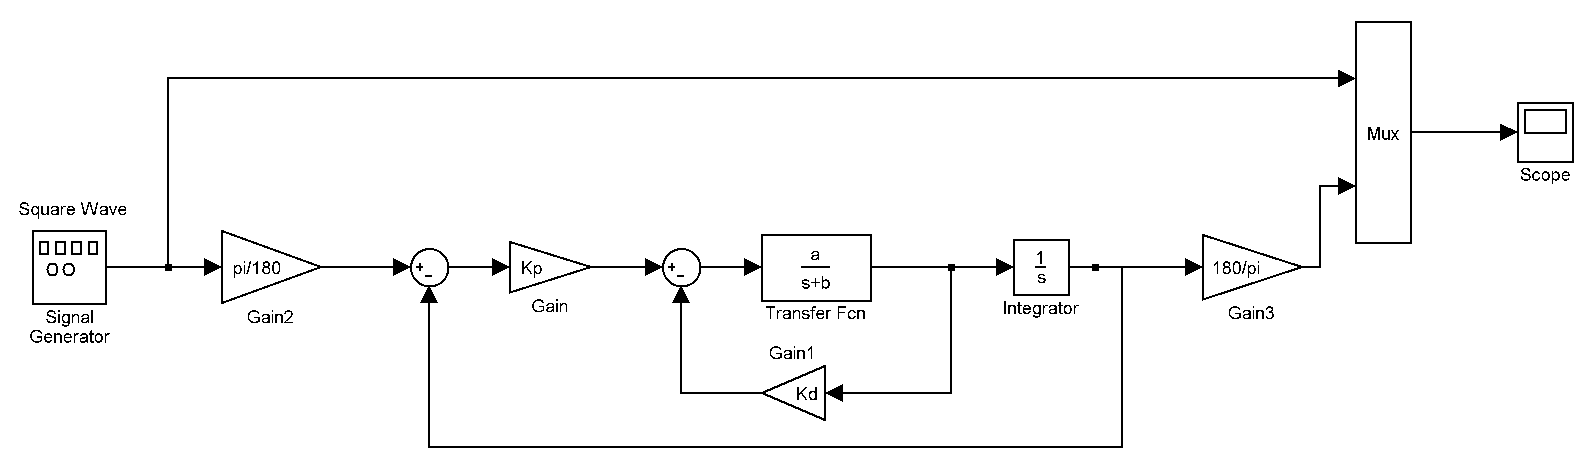
\includegraphics[width=.9\textwidth]{posconprelabPD}
    \caption{\footnotesize
            Simulink model for servo position PD control
            \label{fig.servoPDmodel}
            }
    \end{figure}
    Simulate and use the \verb=plotscope= function to capture the scope's plot and put it in a MATLAB figure plot.  Check to see if the response meets the design requirements.
        \begin{solposcon}
        The solution to this question is provided in Fig.\ \ref{fig.servoPDmodel}.
        \end{solposcon}
\end{enumerate}

All of the prelab calculations, design, and simulation must be completed prior to the laboratory session.  The plant transfer function and controller values must be checked and verified by the instructor prior to implementation.

\begin{thebibliography}{9}
    \bibitem{ogata} Katsuhiko Ogata.  Modern Control Engineering, 4th edition.  Prentice Hall.  2002.
    \bibitem{gears} Giancarlo Genta.  Dynamics of Rotating Systems.  Springer.  2005.
    \bibitem{analogs} Eric Cheever.  Electrical and Mechanical Analogs. \url{http://www.swarthmore.edu/NatSci/echeeve1/Ref/Analogs/ElectricalMechanicalAnalogs.html}
\end{thebibliography}

\Closesolutionfile{PosConSolutions}